%
% $RCSfile: template_editor.tex,v $
%
% Copyright (C) 2002-2008. Christian Heller.
%
% Permission is granted to copy, distribute and/or modify this document
% under the terms of the GNU Free Documentation License, Version 1.1 or
% any later version published by the Free Software Foundation; with no
% Invariant Sections, with no Front-Cover Texts and with no Back-Cover
% Texts. A copy of the license is included in the section entitled
% "GNU Free Documentation License".
%
% http://www.cybop.net
% - Cybernetics Oriented Programming -
%
% http://www.resmedicinae.org
% - Information in Medicine -
%
% Version: $Revision: 1.1 $ $Date: 2008-08-19 20:41:09 $ $Author: christian $
% Authors: Christian Heller <christian.heller@tuxtax.de>
%

\subsection{Template Editor}
\label{template_editor_heading}
\index{CYBOL Template Editor}
\index{Triple-Choice CYBOL Template Editor}

CYBOL applications can be written in an XML-conform way. The use of standard
XML tools to edit and validate CYBOL knowledge templates, at design time, is
therefore possible. An exception are serialised runtime CYBOL models, possibly
made persistent in form of files or in a \emph{Database} (DB), for which XML
conformity has to be given up due to additional markup tokens, as explained in
section \ref{serialised_model_heading}.

Due to the fixed structure of CYBOL knowledge templates (four XML tags, four
XML attributes), more convenient- than standard XML editors shall be
providable. Figure \ref{editor_figure} shows an editor proposal supporting
both, the \emph{Whole-Part-} as well as the \emph{Meta Hierarchy} of CYBOL.
There are three characters indicating the action that a click on a tree node
would evoke:

\begin{itemize}
    \item[+] Open the whole-part hierarchy
    \item[\&] Open the meta hierarchy (properties and constraints)
    \item[-] Close the hierarchy
\end{itemize}

\begin{figure}[ht]
    \begin{center}
        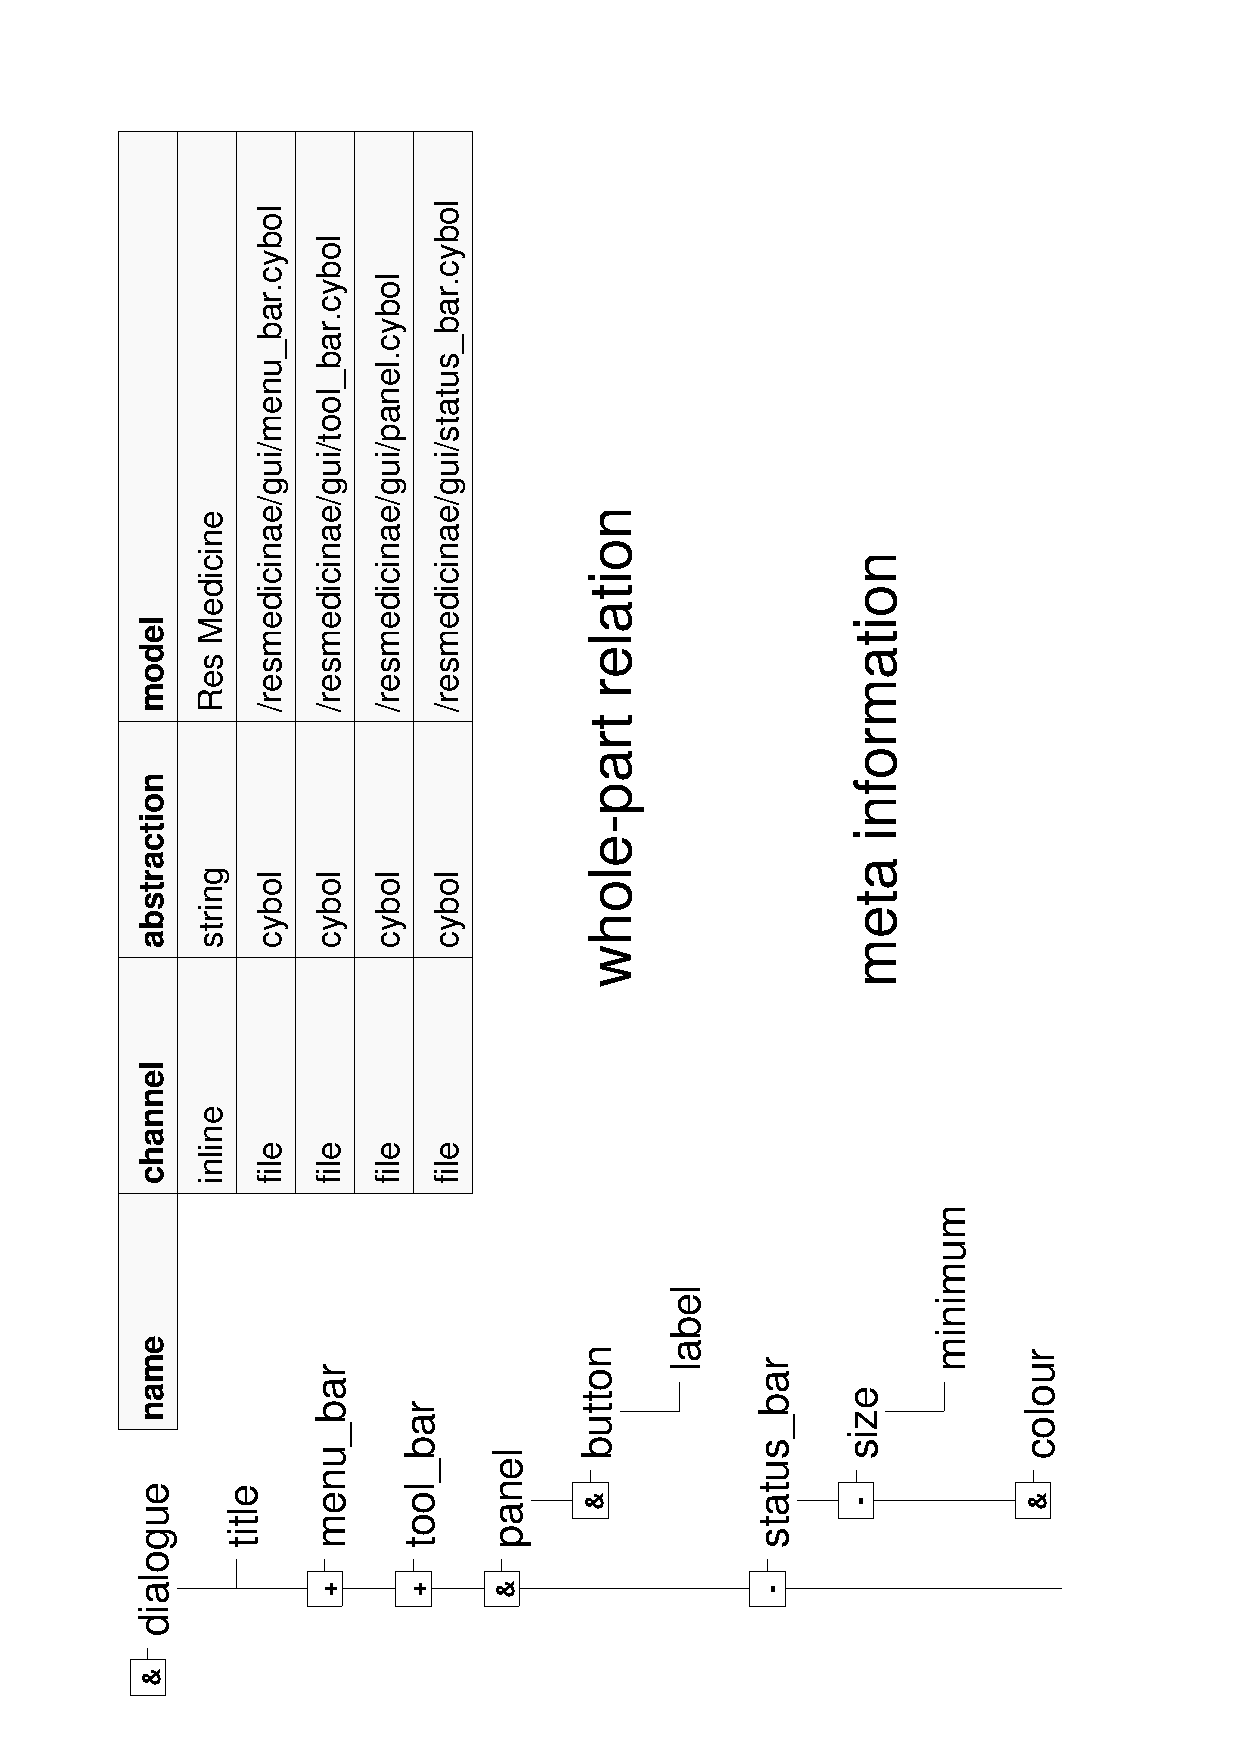
\includegraphics[scale=0.3,angle=-90]{graphic/editor.pdf}
        \caption{CYBOL Editor Supporting Double Hierarchies by Triple Choice}
        \label{editor_figure}
    \end{center}
\end{figure}

The displayed template represents a graphical \emph{dialogue} with its
\emph{title}, \emph{menubar}, \emph{toolbar}, \emph{panel} and \emph{status bar}.
The opened panel node shows its parts, namely \emph{button} and \emph{label}.
The opened status bar node, on the other hand, shows its properties \emph{size}
and \emph{colour}, and additionally the \emph{size}'s \emph{minimum} constraint.
The attribute values of a selected node would be editable in a table like the
one shown on the right-hand side of the figure.

%Prot?g? is an ontology editor and a knowledge-base editor.
%http://protege.stanford.edu/
